\documentclass[a4paper,12pt]{article}
\usepackage{amsmath, amssymb, graphicx, fancyhdr, tcolorbox}
\usepackage{geometry}
\usepackage{fvextra}
\DefineVerbatimEnvironment{verbatim}{Verbatim}{breaklines}
\geometry{a4paper, margin=1in}

% Front Page
\begin{document}
\begin{titlepage}
    \begin{center}
        \vspace*{1cm}
        
        \textbf{42189 Transport system analysis\\Project 1}
        
        \vfill
        
        \textbf{Mikkel Goldchmidt} \\
        Study Number: s183966 \\
        \today
        
        \vfill
        
        \begin{tcolorbox}[colframe=black, colback=gray!10, width=0.8\textwidth, sharp corners]
        \textbf{Remark:} 
        This project is written in its entirety by Mikkel Goldschmidt, by prior agreement with the course responsible. 
        Generative AI has been used during the proces of understanding the course in general.
        Further GitHub Copilot has been used to write smaller snippets of code. 
        Finally it has been used for proof reading sections of the report. A log of all use of AI has been kept and can be provided upon request.
        \end{tcolorbox}
    \end{center}
\end{titlepage}

\section{Exercise 1: Mode Choice Model Estimation}

\subsection{Task 1: Estimation}
Both models have negative signs for higher travel times and travel costs, which is as expected. Both of them also have a negative coefficient for taking public transport, which is in general less convenient due to the externally dictated departures and arrivals along with having to deal with all the other passengers. The only difference in sign between the two models is on biking, where model 2 shows it as better than walking (positive coefficient sign) and model 1 shows it as worse (negative coefficient sign). This does not on its own exclude any of the models, as it is not obvious if people in general like biking or walking more.

The most significant change between the two is the coefficient in front of the cost variable. That is as expected, as the values are significantly lower after the log function having been applied.

Neither model is a restricted version of the other, thus we cannot do the likelihood ratio test. However, since the two models have exactly the same amount of parameters, we can simply compare the two LL values. This approach leaves us with model 2 as the better model, as it has a larger Log-Likelyhood (read from the bottom of the model summary).

\subsection{Task 2: Market Share Calculation}
In the following, the data has been saved in the variable \texttt{data} as a pandas DataFrame

To calculate the the utilities for each mode and individual, 
we used the utility function
$$
V_{ni} = k_{ni} + a\cdot \ln(\text{cost}_{ni}) + b \cdot \text{time}_{ni}
$$
with the values read from the model R summary of model 2.

With code like the following line, to calculate the utility
\begin{verbatim}
data["UtilityBike2"] = m2["k2"] + m2["b"]*data["TT2"] + m2["a"]*np.log(data["TC2"])
\end{verbatim}
and code like the following to calculate the probability
\begin{verbatim}
data["ProbabilityBike2"] = np.exp(data["UtilityBike2"]) / np.exp(data[["UtilityWalk2", "UtilityBike2", "UtilityCar2", "UtilityPublic2"]]).sum(axis=1)
\end{verbatim}

Now having calculated the probabilities for each mode, we can extract the ones for observation 1.
\begin{verbatim}
first_row_probabilities = data.loc[0, ['ProbabilityWalk2', 'ProbabilityBike2', 'ProbabilityCar2', 'ProbabilityPublic2']]
\end{verbatim}
will then yield:
\begin{verbatim}
ProbabilityWalk2      0.042564
ProbabilityBike2      0.146982
ProbabilityCar2       0.756599
ProbabilityPublic2    0.053855
\end{verbatim}

The market shares can be compared as follows:
\begin{verbatim}
predicted_walking_2 = data['ProbabilityWalk2'].sum()
predicted_biking_2 = data['ProbabilityBike2'].sum()
predicted_car_2 = data['ProbabilityCar2'].sum()
predicted_public_2 = data['ProbabilityPublic2'].sum()
total = predicted_walking_2 + predicted_biking_2 + predicted_car_2 + predicted_public_2

predicted_distribution_2 = pd.DataFrame({
    'Mode': ['Walking', 'Biking', 'Car', 'Public Transport'],
    'Predicted Distribution': [predicted_walking_2, predicted_biking_2, predicted_car_2, predicted_public_2] / total
})
\end{verbatim}
which will yield the following market shares:
\begin{verbatim}
| Mode             |   Predicted Distribution |
|:-----------------|-------------------------:|
| Walking          |                0.193519  |
| Biking           |                0.222669  |
| Car              |                0.547886  |
| Public Transport |                0.0359261 |
\end{verbatim}

We see that this person, is more predicted more likely to take the car.
This is also the decision that the person actually took when looking in the table.


\subsection{Task 3: Value of Time}
The value of time is defined as utility derived with respect to travel time divided by the utility derived with respect to travel cost.
For model two, the one derived with respect to travel time, is easily recognized as $b$.
The one with respect to travel cost is different, as it has the natural logarithm as well.
Thus we will calculate:
$$
\dfrac{\delta V_{ni}}{\delta c_{ni}} = \dfrac{\delta \left( k_i + a\ln(c_{ni}) + b\cdot t_{ni} \right)}{\delta c_{ni}} = a \dfrac{\delta \ln(c_{ni})}{\delta c_{ni}} = \frac{a}{c_{ni}}
$$
The value of time can then be calculated as
$$
VTT_{ni}= \dfrac{\delta V_{ni}}{\delta t_{ni}} / \dfrac{\delta V_{ni}}{\delta c_{ni}} = b / \left(\frac{a}{c_{ni}}\right) = c_{ni} \frac{b}{a}
$$

Calculating this is fairly easy, as the dataset has a travel cost column.
The average value for this over each customer is then found to be 0.42 DKK per minute. 
The maximum value found is 5.25 and minimal almost 0 with a median quite a bit below the average at 0.16. 
These values don't seem a lot off - they are for the most part clearly below the salary of the average worker whilst still being a not insignificant amount of money. 
However, the model postulates that the VTT is directly proportional to the travel cost, which seems a bit odd and counter to what I would have guessed. I would have expected a person with a long expensive trip to care less about getting it prolonged a bit than a person who has a short (and thus less expensive) trip.

\subsection{Task 4: Elasticities Analysis}
\subsubsection{Direct Elasticity}
The direct elasticity with respect to $x_{ni}$ can by (6.20) be calculated as
$$
E^{x_{ni}}_{ii} =
\dfrac { \partial V_{ni} } { \partial x_{ni} }
x_{ni} (1 - P_{ni})
$$
where $V_{ni}$ is the [[utility function]] and $P_{ni}$ is the probability for $n$ with mode $i$. 

These can be calculated for cost :
$$
E^{c_{ni}}_{ii} =
\dfrac { \partial V_{ni} } { \partial c_{ni} }
c_{ni} (1 - P_{ni}) 
= \frac{a}{c_{ni}}c_{ni}(1 - P_{ni}) = a(1 - P_{ni})
$$
and
$$
E^{t_{ni}}_{ii} =
\dfrac { \partial V_{ni} } { \partial t_{ni} }
t_{ni} (1 - P_{ni})
= b t_{ni}(1-P_{ni})
$$
for time.

That yields the following elasticities:
\begin{verbatim}
| Mode   |   TimeElasticity |   PriceElasticity |
|:-------|-----------------:|------------------:|
| Walk   |       -0.441012  |         -0.33221  |
| Bike   |       -0.315335  |         -0.338125 |
| Car    |       -0.0657483 |         -0.180048 |
| Public |       -0.569098  |         -0.427734 |
\end{verbatim}

These are fairly sensible, as they are all negative indicating that 
the probability of choosing a mode decreases if it either gets more expensive or takes longer time.

\subsubsection{Cross Elasticity}
The cross elasticity for change in mode $i$ dependent on change in $j$ for $n$  is shown in (6.21) with respect to variable $x$ to be
$$
E^{x_{nj}}_{nij} = -\dfrac{\partial V_{nj}}{\partial x_{nj}}
x_{nj} P_{nj}
$$
since the derivative on the [[utility function]] is only different from their example with (6.22) and (6.23) by a constant, their derivations can be used to conclude that cross elasticity for the cost can be calculated as
$$
E^{c_{nj}}_{nij} =-aP_{nj}
$$
and for the time
$$
E^{t_{nj}}_{nij} =-b t_{nj} P_{nj}
$$

note that neither of these are dependent on $i$, that is the analysed mode. We therefor have a change in any $j$ will change the other three modes with the same elasticity as seen in the table below:

\begin{verbatim}
| Mode   |   TimeCrossElasticity |   PriceCrossElasticity |
|:-------|----------------------:|-----------------------:|
| Walk   |             0.0947405 |              0.11679   |
| Bike   |             0.074305  |              0.110875  |
| Car    |             0.174241  |              0.268952  |
| Public |             0.033231  |              0.0212658 |
\end{verbatim}

The above should be read as, if the driving time for cars increase by 10\%, the usage of all the others will icrease roughly 1.74\%.
These are also fairly sensible, as they are all positive indicating that
the probability of choosing a mode increases if another mode gets more expensive or takes longer time.

\subsection{Task 5: Model Specification and Gender Differences}
Comparing the genders, we see that they seem to walk and bike the same, but the men more often take cars and women more often public transport compared to the other gender.

To assess Utility function 3, we consider if the signs of the parameters are sensible.
They seem to almost the same as the ones in utility function 2, making it quite plausible.
If we wanted to evaluate if the model was better, we could use the likelihood ration test to see if the new model match the data better.

When using the new utility function, it will produce exactly the same prediction of market shares when run on the entire population.
This is seen both by the actual calculation done, but it is actually known directly from the slides from week 4 under the "Alternative specific constants" where this result is argued from the way that the models have been chosen (they always sum to the underlying distribution of the data).


\subsection{Task 6: Scenario Application - Green Car Introduction}
A way to do this prediction, is to simply calculate the probabilities for each individual again with a new option of the "Green car" added.
That car will just have $1.2$ times the cost of travel and $\frac{1}{1-0.2}=1.25$ times the travel time (the speed is $20\%$ slower).

This yields the following prediction for market shares:

\begin{verbatim}
| Mode             | Market Share model 3 | Predicted Market Share |
| :--------------- | -------------------: | ---------------------: |
| Walking          |             0.193519 |               0.214999 |
| Biking           |             0.222669 |               0.197838 |
| Car              |             0.547886 |               0.341606 |
| Public Transport |            0.0359261 |              0.0179565 |
| Green Car        |                    0 |                 0.2276 |
\end{verbatim}

Obviously this way of modelling the new car is sub optimal. It does not at all take into account, that the new car is "greener" and no one in their right mind would pay more for an expensive car just for the privilege of driving slower. 
To make the results better, one could for instance introduce a "green" variable to the model, that would apply to all non-fossil fuel vehicles in the original model to try to estimate to what degree the travelers prioritize green forms of transportation. If a reliable version of such a model could be constructed, one could probably make a better prediction.

\section{Exercise 2: Trip Distribution Modelling}

\subsection{Task 1: Implementing the Model}
\subsubsection{Mode choice utility function}
As calculating the actual values of the utility functions, take of quite a lot of space with all combinations of districts and modes of transportation, the actual numbers are left for the appendix.
However, below plots showing a heatmap of the utilities for car driving and public transport between districts is shown in figure \ref{fig:car_public_utility}.
\begin{figure}
    \centering
    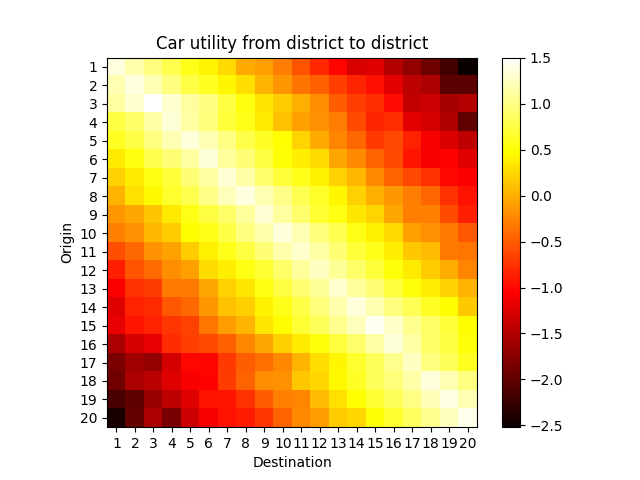
\includegraphics[width=0.4\textwidth]{car_utility.png}
    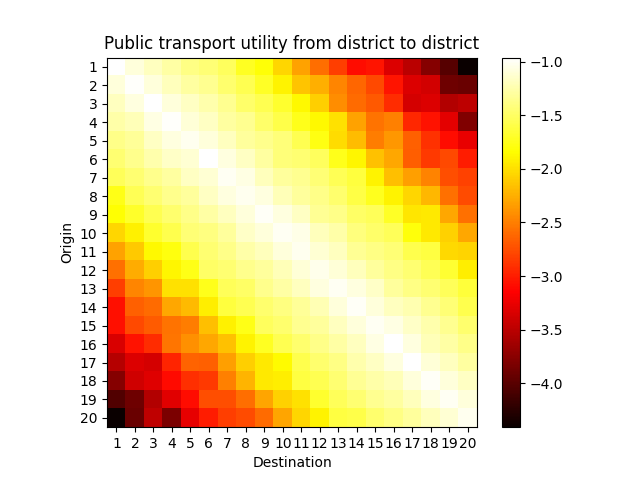
\includegraphics[width=0.4\textwidth]{public_utility.png}
    \caption{Heatmap of the utility for car driving and public transport between districts}
    \label{fig:car_public_utility}
\end{figure}

\subsubsection{Conditional mode choice probabilities $P_i(m|d)$}
To calculate the conditional mode choices, we use formua (7.3).
That is the following formula:
$$
P_i(m|d) = \dfrac{\exp(V_i(m,d))}{\sum_{m'} \exp(V_i(m',d))}
$$
which is implemented in the code below.

\begin{verbatim}
df_trips['U_walk'] = 0
df_trips['U_bike'] = 0
df_trips['U_car'] = 0
df_trips['U_carpool'] = 0
df_trips['U_public_transport'] = 0

for index, row in df_trips.iterrows():
    d_from = row['ResiZone']
    d_to = row['DestZone']
    df_trips.at[index, 'U_walk'] = utility_walk(d_from, d_to)
    df_trips.at[index, 'U_bike'] = utility_bike(d_from, d_to)
    df_trips.at[index, 'U_car'] = utility_car(d_from, d_to)
    df_trips.at[index, 'U_carpool'] = utility_carpool(d_from, d_to)
    df_trips.at[index, 'U_public_transport'] = utility_public_transport(d_from, d_to)

# Calculate the sum of the exponentials for each district combination
df_trips['sum_exp'] = df_trips[['U_walk', 'U_bike', 'U_car', 'U_carpool', 'U_public_transport']].apply(lambda x: np.exp(x)).sum(axis=1)

# Calculate the conditional mode choice probabilities
# using formula (7.3)
df_trips['P_walk'] = np.exp(df_trips['U_walk']) / df_trips['sum_exp']
df_trips['P_bike'] = np.exp(df_trips['U_bike']) / df_trips['sum_exp']
df_trips['P_car'] = np.exp(df_trips['U_car']) / df_trips['sum_exp']
df_trips['P_carpool'] = np.exp(df_trips['U_carpool']) / df_trips['sum_exp']
df_trips['P_public_transport'] = np.exp(df_trips['U_public_transport']) / df_trips['sum_exp']
\end{verbatim}

\paragraph{Individual living in district 1 going to district 2}
Extracting the probabilities for an individual living in district 1 going to district 2, we get the following probabilities:
\begin{verbatim}
|    P_walk |   P_bike |    P_car |   P_carpool |   P_public_transport |
|----------:|---------:|---------:|------------:|---------------------:|
| 0.0336238 | 0.265739 | 0.556988 |   0.0859606 |            0.0576886 |
\end{verbatim}


\subsubsection{Destination choice utility function}
A ranked list of $V_n$ of all 20 districts has been calculated and can be seen in the appendix.
They have been calculated using the formula.
Notable from the list is that the three highst ranking are 12, 20 and 15.
The lowest are 9, 17 and 13.

\subsubsection{Destination choice probabilities $P_i(d)$}
To caculate this formula (7.4) is used, which gives 
$$
P_i(d) = \dfrac{\exp(V_i(d) + I(d))}{\sum_d \exp(V_i(d) + I(d))}
$$
where
$$
I(d) = \mu \ln\left(\sum_m \exp\left(\dfrac{V(m|d)}{\mu}\right)\right)
$$
Note that in this implementation, I'm incorporating the $\mu$ into the $I$.
In some of the slides, this is done in the $P_i$ calculation, but I have chosen to follow the standard from the book instead of the slides.

As the Task does not specify to report numbers from this calculation (a heatmap of it can however be seen in figure \ref{fig:destination_choice}), 
it will be left in the appendix for Exercise 2 at the codeblock calculating it, that looks like the following:
\begin{verbatim}
for n in districts:
    for d in districts:
        W = destination_utility(n, d)
        
        sum_exp = 0
        for d_prime in districts:
            W_prime = destination_utility(n, d_prime)
            I_prime = df_trips[(df_trips["ResiZone"] == n) & (df_trips["DestZone"] == d_prime)]["I"].values[0]
            sum_exp += np.exp(W_prime + I_prime)
        
        I_nd = df_trips[(df_trips["ResiZone"] == n) & (df_trips["DestZone"] == d)]["I"].values[0]
        
        df_trips.loc[(df_trips["ResiZone"] == n) & (df_trips["DestZone"] == d), "P_dest"] = np.exp(W + I_nd) / sum_exp
\end{verbatim}

\begin{figure}[h]
    \centering
    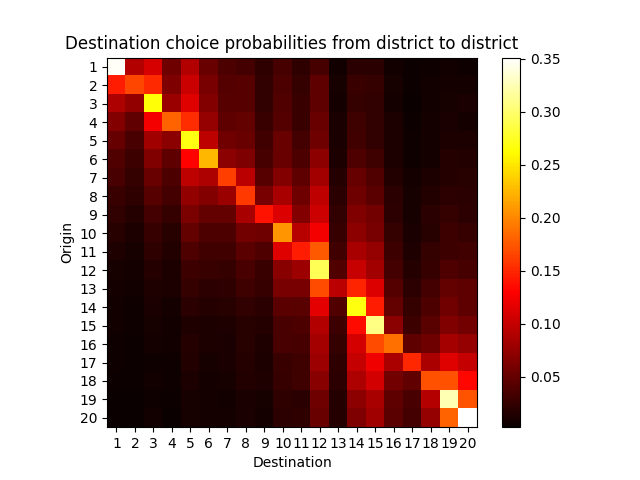
\includegraphics[width=0.7\textwidth]{destination_choice.png}
    \caption{Heatmap of the destination choice probabilities}
    \label{fig:destination_choice}
\end{figure}

\subsubsection{Average mode shares}
The average mode shares can be calculated as the sum of the probabilities for each mode divided by the number of trips.
This is done in the following code block:
\begin{verbatim}
walking_amount = pd.DataFrame(index=districts, columns=districts)
biking_amount = pd.DataFrame(index=districts, columns=districts)
car_amount = pd.DataFrame(index=districts, columns=districts)
carpool_amount = pd.DataFrame(index=districts, columns=districts)
public_transport_amount = pd.DataFrame(index=districts, columns=districts)

for d_from in districts:
    for d_to in districts:
        # Get the amount of people going from district i to district j
        travel_count = travelers.at[d_from, d_to]

        # Get the mode choice probabilities for the route
        P_walk = df_trips[
            (df_trips["ResiZone"] == d_from) & (df_trips["DestZone"] == d_to)
        ]["P_walk"].values[0]
        P_bike = df_trips[
            (df_trips["ResiZone"] == d_from) & (df_trips["DestZone"] == d_to)
        ]["P_bike"].values[0]
        P_car = df_trips[
            (df_trips["ResiZone"] == d_from) & (df_trips["DestZone"] == d_to)
        ]["P_car"].values[0]
        P_carpool = df_trips[
            (df_trips["ResiZone"] == d_from) & (df_trips["DestZone"] == d_to)
        ]["P_carpool"].values[0]
        P_public_transport = df_trips[
            (df_trips["ResiZone"] == d_from) & (df_trips["DestZone"] == d_to)
        ]["P_public_transport"].values[0]

        # Calculate the amount of people going by each mode
        walking_amount.at[d_from, d_to] = travel_count * P_walk
        biking_amount.at[d_from, d_to] = travel_count * P_bike
        car_amount.at[d_from, d_to] = travel_count * P_car
        carpool_amount.at[d_from, d_to] = travel_count * P_carpool
        public_transport_amount.at[d_from, d_to] = travel_count * P_public_transport

# Sum the amount of people going by each mode
walking_amount = walking_amount.astype(float)
biking_amount = biking_amount.astype(float)
car_amount = car_amount.astype(float)
carpool_amount = carpool_amount.astype(float)
public_transport_amount = public_transport_amount.astype(float)

# Sum the amount on both axis
walking_amount = walking_amount.sum(axis=0).sum(axis=0)
biking_amount = biking_amount.sum(axis=0).sum(axis=0)
car_amount = car_amount.sum(axis=0).sum(axis=0)
carpool_amount = carpool_amount.sum(axis=0).sum(axis=0)
public_transport_amount = public_transport_amount.sum(axis=0).sum(axis=0)
\end{verbatim}
this yields the following amount of people going by each mode:
\begin{verbatim}
Walking: 5958.0
Biking: 19565.0
Car: 68606.0
Carpool: 11378.0
Public transport: 8980.0
\end{verbatim}
which can be divided by the total amount of people to get the market shares:
\begin{verbatim}
Market shares:
Walking: 5.2 %
Biking: 17.1 %
Car: 59.9 %
Carpool: 9.9 %
Public transport: 7.8 %
\end{verbatim}

\subsection{Task 2: Model Estimation and Calibration}
To solve this task, I needed to abstract out the calculation of market shares into a function, where the initial parameters could be changed.
This is seen in the notebook in the appendix where a function \texttt{calculate\_market\_shares} is defined.
This function is then used to calculate the market shares given a set of alphas.
The model is altered slightly to, adding an alpha paramter to the public transport (initialized as $0$), which was the baseline the other parameters where chosen in relation to before.

% array([ 1.24486936,  1.81193381,  0.53930656, -0.61750051,  0.30535498])
Algorithm 14.1 is then run a few times, yielding the new value for the constants
\begin{table}[h!]
\centering
\begin{tabular}{|c|c|c|}
    \hline
    \textbf{Parameter} & \textbf{Old value} & \textbf{New value} \\
    \hline
    $k_{\text{walk}}$ & 1.5 & 1.24486936 \\
    $k_{\text{bike}}$ & 2 & 1.81193381 \\
    $k_{\text{car}}$ & 0.5 & 0.53930656 \\
    $k_{\text{carpool}}$ & -0.5 & -0.61750051 \\
    $k_{\text{public}}$ & 0 & 0.30535498 \\
    \hline
\end{tabular}
\caption{Comparison of old and new parameter values}
\label{tab:parameter_values}
\end{table}

Using these parameters in the model now almost perfectly matches the market shares.

\subsection{Task 3: Analyse model sensitivity}
Using the function defined earlier (with a tiny hack to change the original data table),
the market shares can be calculated forthe four different scenarios fairly easilty.
FOr instance, calculating the increased car cost market shares are done using the line
\begin{verbatim}
cc_increased = calculate_market_shares(alphas_2, increase_param='cc')
\end{verbatim}
Doing this for all the scenarios, yields a table like the one asked for in Table \ref{tab:market_shares}.
\begin{table}[h!]
    \centering
    \begin{tabular}{|l|c|c|c|c|}
        \hline
        & \textbf{cc increased} & \textbf{ct increased} & \textbf{pc increased} & \textbf{pt increased} \\
        \hline
        Walk & 0.0413514 & 0.0415657 & 0.0405613 & 0.0404054 \\
        \hline
        Bike & 0.145521 & 0.146312 & 0.142884 & 0.142304 \\
        \hline
        Car & 0.614353 & 0.617704 & 0.628686 & 0.626184 \\
        \hline
        Carpool & 0.0902107 & 0.0849128 & 0.0890926 & 0.0887403 \\
        \hline
        Public transport & 0.108564 & 0.109506 & 0.0987752 & 0.102367 \\
        \hline
    \end{tabular}
    \caption{Market shares for different scenarios}
    \label{tab:market_shares}
\end{table}

To get the elasticities from this, the difference in market shares are calculated and divided by the change in the parameter.
The elasticities are then calculated as seen in Table \ref{tab:elasticities}.
\begin{table}[h!]
    \centering
    \begin{tabular}{|l|c|c|c|c|}
        \hline
        & \textbf{cc increased} & \textbf{ct increased} & \textbf{pc increased} & \textbf{pt increased} \\
        \hline
        Walk & 0.26\% & 0.31\% & 0.06\% & 0.03\% \\
        \hline
        Bike & 0.26\% & 0.31\% & 0.07\% & 0.03\% \\
        \hline
        Car & -0.14\% & -0.09\% & 0.09\% & 0.05\% \\
        \hline
        Carpool & 0.22\% & -0.38\% & 0.09\% & 0.05\% \\
        \hline
        Public transport & 0.21\% & 0.3\% & -0.71\% & -0.37\% \\
        \hline
    \end{tabular}
    \caption{Elasticities for different scenarios}
    \label{tab:elasticities}
\end{table}

The elasticities seem to all have appropriate signs. 
When car driving time and cost increases, the car driving market share decreases.
The same goes for public transport with increased cost and time.
All others rise under the same conditions, which is also as expected.

\subsection{Task 4: Apply the model}
To do the pivot, we calculate the base model and the sc model, using the function defined earlier.
Then relative changes in the model is calculated by subtracting the two elementwise and dividing by the base model.
The differences are then multiplied with the original data to get the new values.
This is done in the following code block:

\begin{verbatim}
df_model_base = calculate_market_shares(alphas_2, return_df=True)
df_model_sc = calculate_market_shares(alphas_2, pc=10, return_df=True)

df_relative_change = (
    df_model_sc[["P_walk", "P_bike", "P_car", "P_carpool", "P_public_transport"]]
    - df_model_base[["P_walk", "P_bike", "P_car", "P_carpool", "P_public_transport"]]
) / df_model_base[["P_walk", "P_bike", "P_car", "P_carpool", "P_public_transport"]]

df_od['trip_w_sc'] = df_od['trip_w'] * (1 + df_relative_change['P_walk'])
df_od['trip_b_sc'] = df_od['trip_b'] * (1 + df_relative_change['P_bike'])
df_od['trip_c_sc'] = df_od['trip_c'] * (1 + df_relative_change['P_car'])
df_od['trip_cp_sc'] = df_od['trip_cp'] * (1 + df_relative_change['P_carpool'])
df_od['trip_p_sc'] = df_od['trip_p'] * (1 + df_relative_change['P_public_transport'])
\end{verbatim}

This yields the following table of predicted demands after the introduced scenario in Table \ref{tab:predicted_demands}.

\begin{table}[h!]
    \centering
    \begin{tabular}{|l|r|r|}
        \hline
        \textbf{Mode} & \textbf{Pre scenario} & \textbf{Post scenario} \\
        \hline
        Walk & 13,304 & 13,109 \\
        \hline
        Bike & 46,879 & 45,970 \\
        \hline
        Car & 205,833 & 194,322 \\
        \hline
        Carpool & 29,161 & 27,773 \\
        \hline
        Public transport & 35,097 & 48,523 \\
        \hline
    \end{tabular}
    \caption{Predicted demands before and after the scenario}
    \label{tab:predicted_demands}
\end{table}

Unsurprisingly the public transport demand increases a lot by the decreased cost.
The predicted demand is expected to increase by about 13000 trips.

\end{document}

